% Section content template for individual Educative lessons
% This file contains the actual content for a specific section
% Generated from Educative API section content

% Section: Sequence Diagram for the Amazon Locker Service
% Section ID: 5436453903663104
% Section Slug: sequence-diagram-for-the-amazon-locker-service
% Generated: 2025-12-11T15:17:22.483541

Sequence diagrams are a great way to understand the interactions between different entities and objects in the system. We can create different sequence diagrams for our Amazon Locker system. We will create a sequence diagram for returning a package in this lesson.

\subsection{Return package}\label{VGX1aCapGu5xp6wNV0JSj}
\\
The sequence diagram for the package return should have the following actors and objects that will interact with each other:
\\
\textbf{Actors / Participants}

\begin{itemize}
\item
\protect\phantomsection\label{ATBX5-0xOFVUVrQ_LIRfp}
Customer (the person returning the package)
\item
\protect\phantomsection\label{Ar1sJHHkLSFq79YKLIlOy}
LockerService (the central system that manages lockers and OTPs)
\item
\protect\phantomsection\label{6ge_YlvHqB9_TEc-BBzDD}
Locker (an individual locker unit)
\item
\protect\phantomsection\label{voqir6xc6Siep1iX4nkXE}
Notification (responsible for sending OTPs and messages to the customer)
\end{itemize}
\\
Here are the steps in the return package interaction:

\begin{enumerate}
\item
\protect\phantomsection\label{ySqBpb7txW-jR0s3hsPKu}
The customer asks the system to initiate a package return.
\item
\protect\phantomsection\label{d81jObrz4P_dy3HLomzFB}
System checks approval:

\begin{enumerate}
\item
If the return is \emph{denied}, the system immediately notifies the customer, and the process ends.
\item
If the return is approved, proceed to the next step.
\end{enumerate}
\item
\protect\phantomsection\label{ed-c4yHB1Sxq8f2xUj5cX}
The system finds the first free locker and reserves it.
\item
\protect\phantomsection\label{m4RVsB7b-PROnVNA6Ujvz}
Send and verify OTP:

\begin{enumerate}
\item
The system sends the customer a one-time passcode (OTP).
\item
The customer submits the OTP back to the system.
\item
If the code is \emph{invalid or expired}, the system informs the customer and stops.
\item
If the code is valid, move on to the next step.
\end{enumerate}
\item
\protect\phantomsection\label{mM2MqDnTEJ_WQ6u8bv0b4}
Assign locker and place package:

\begin{enumerate}
\item
The system assigns the reserved locker to the customer (marks it as booked).
\item
The customer places the package into that locker, completing the return.
\end{enumerate}
\item
\protect\phantomsection\label{7n4DlLz4cIdqZztv5qORl}
The process is finished. Once the package is in place, no further action is needed.
\end{enumerate}
\\
Based on the order above, the sequence diagram of package return in the Amazon Locker system is given below:

\begin{figure}[htbp]
 \centering
 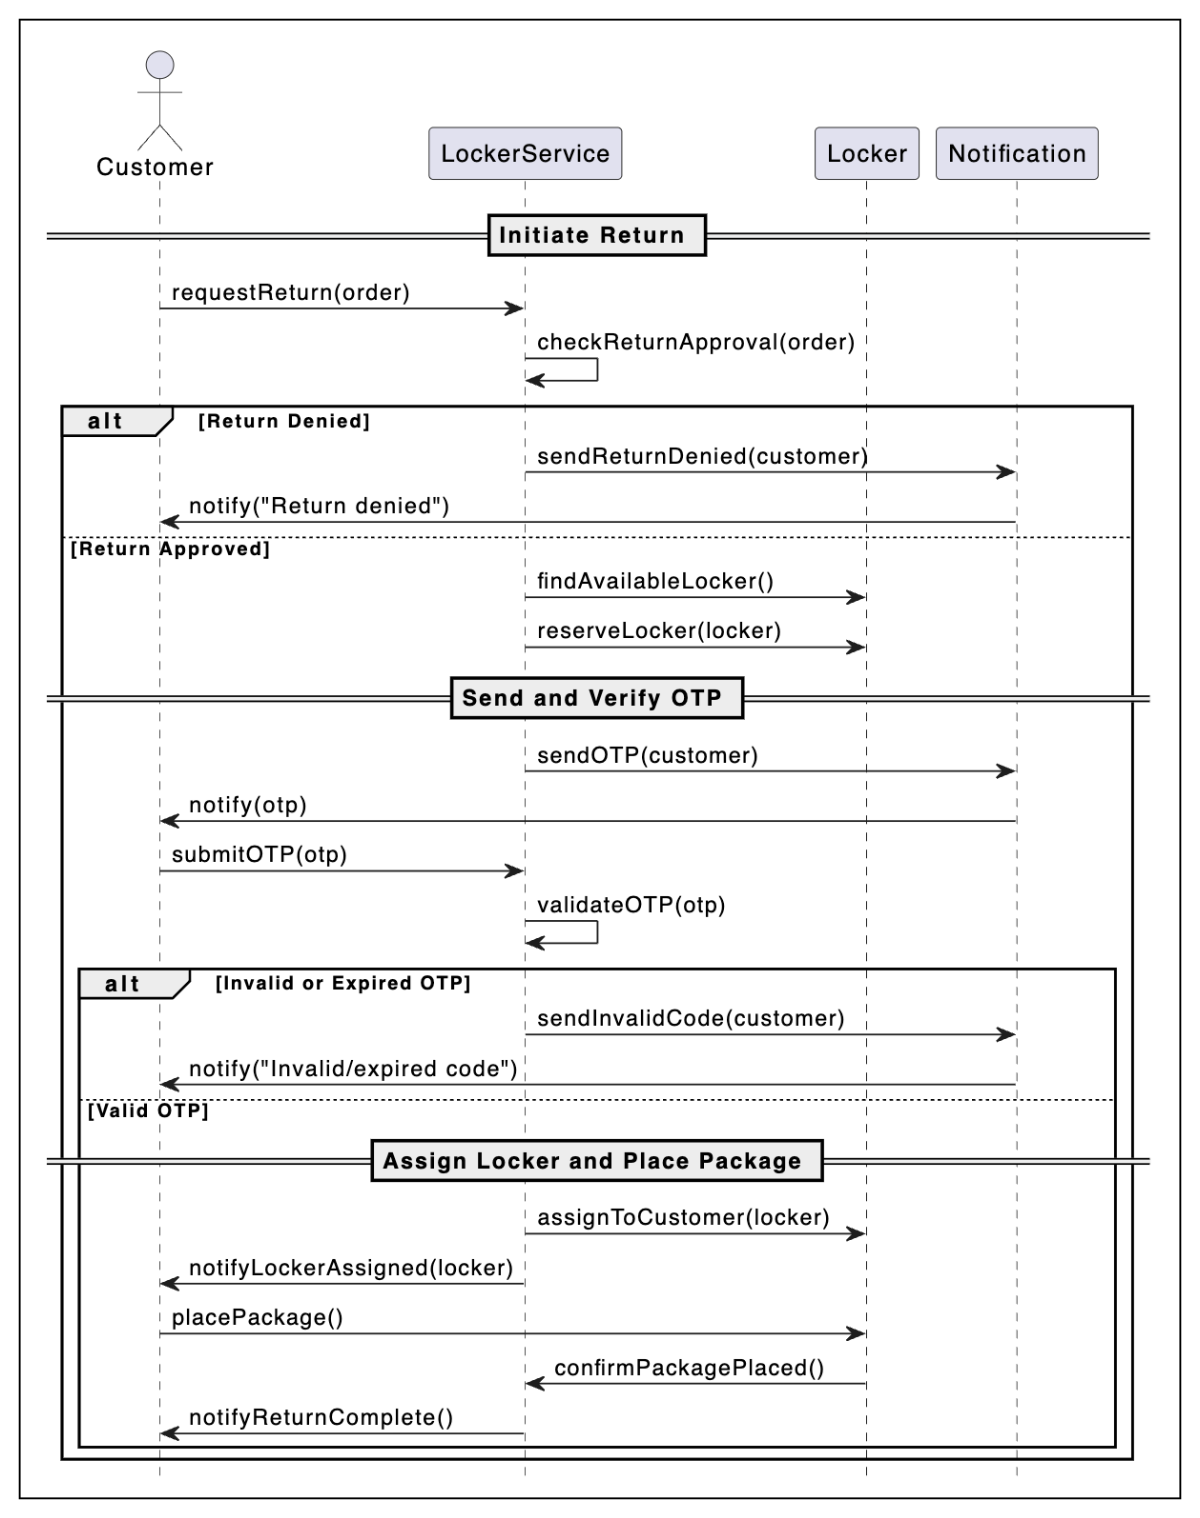
\includegraphics[width=0.5\textwidth]{Images/chapter_10/section_5436453903663104/4903139374137344.png}
 \caption{The sequence diagram for returning a package}
\end{figure}

Next, let's examine the activity diagrams for the Amazon Locker system to understand its control flow.

% End of section content